% Generated by experiments/paper/fig_triage.py; do not edit.
\begin{figure*}[t]
\centering
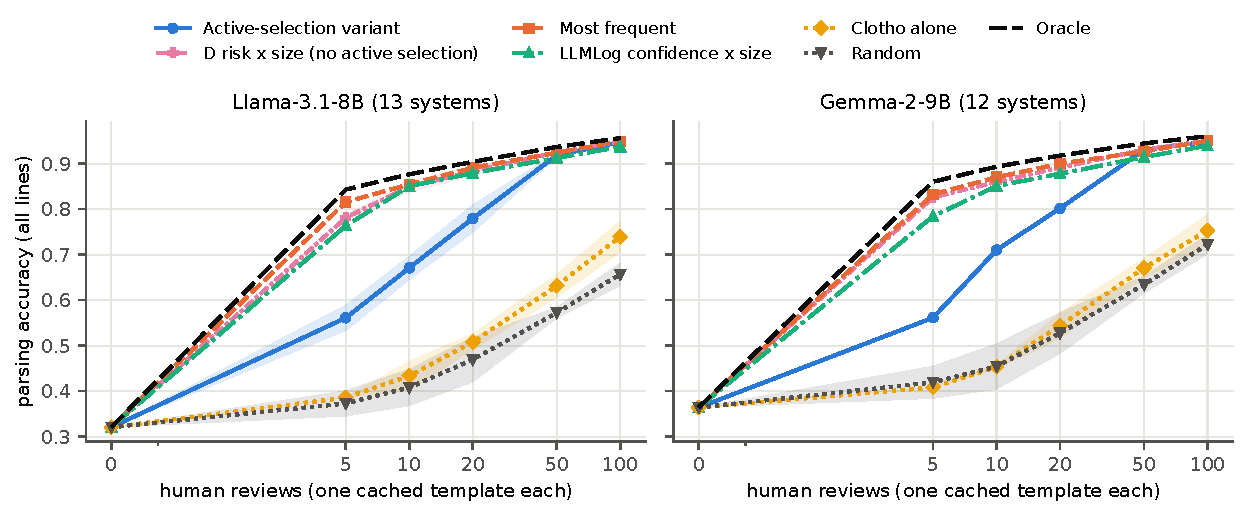
\includegraphics[width=\textwidth]{figures/triage_reviews.pdf}
\caption{Parsing accuracy of a cached LLM log parser versus the number of human reviews. Per system, the first 50,000 Loghub-2.0 lines in log order; Drain (Loghub-2.0 settings) groups lines, the LLM parses the first line of each new group (rules\_template, greedy) and the template is cached for the group. A review replaces one cached template with the group's correct template. Macro mean over systems, mean over 5 seeds (band: $\pm$ std over seeds). Active-selection variant: cross-system prior (D) refit with verdicts, Clotho-style uncertainty and diversity selection among the top-$M$ by risk $\times$ lines; D risk $\times$ lines: top risk $\times$ lines; Oracle: wrong templates by lines they break.}
\label{fig:triage-reviews}
\end{figure*}
